\subsection{传递性}

设 X 是局部紧空间，局部紧群 H 通过 \((x,\xi)\mapsto x\xi\) 在其中连续且 逆紧地从右作用（\((x\in\mathbf{X},\xi\in\mathbf{H})\)）。设 \(H'\) 是 H 的闭子群；则 \(H'\) 也在 X 上连续且 逆紧地从右作用。记 \(\pi,\pi',p\) 分别为从 X 到 X/H、从 X 到 \(X/H'\)、以及从 H 到 \(H/H'\) 的典范映射。

设 \(\beta, \beta'\) 分别是 H、H' 上的左 Haar 测度；假设 \(\Delta_{\mathrm{H}}\) 与 \(\Delta_{\mathrm{H}'}\) 在 H' 上一致；于是可在 H/H' 上构造关于 H 左不变的测度 \(\beta / \beta'\)（No.~6, Th. 3）。另一方面，设 \(\mu\) 是 X 上满足

\[
\delta (\xi) \mu = \Delta_ {\mathrm{H}} (\xi) \mu
\]

对于 \(\xi \in \mathbf{H}\)；则可构造测度 \(\mu / \beta\)，定义在 \(\mathrm{X} / \mathrm{H}\) 上，以及测度 \(\mu / \beta'\)，定义在 \(\mathrm{X} / \mathrm{H}'\) 上（No.~2, Prop. 4）。我们将把 \(\mu / \beta'\) 写成关于 \(\mu / \beta\) 的积分，其中被积的是一个取值于 \(\mathrm{X} / \mathrm{H}'\) 上测度的族，以 \(\mathrm{X} / \mathrm{H}\) 的点为指标。当 \(\mathrm{H}' = \{e\}\) 时，我们又回到 No.~3 的情形。

\pandocbounded{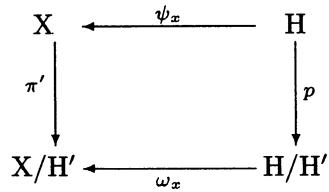
\includegraphics[keepaspectratio]{images/part001_c0ba5876.jpg}}

映射 \((x,\xi)\mapsto\pi'(x\xi)\) 从 \(X\times H\) 到 \(X/H'\) 连续；由于 \(\pi'(x\xi)=\pi'(x\xi\xi')\) 对所有 \(\xi'\in H'\) 成立，该映射通过取商定义了从 \(X\times(H/H')\) 到 \(X/H'\) 的连续映射；因此，对于 X 中每个固定的 x，通过取商得到偏映射 \(\omega_{x}\)，从 \(H/H'\) 到 \(X/H'\)，它由 H 到 X 的映射 \(\psi_x: \xi \mapsto x\xi\) 导出。注意 \(\psi_{x\xi} = \psi_x \circ \gamma_H(\xi)\)，因而 \(\omega_{x\xi} = \omega_x \circ \gamma_{\mathrm{H/H'}}(\xi)\)，对所有 \(\xi \in \mathrm{H}\) 成立。

引理 7. --- 设 K 是 X/H' 的紧子集，L 是 X 的紧子集。则 \(\bigcup_{x\in\mathbf{L}}\omega_{x}^{-1}(\mathbf{K})\) 在 H/H' 中相对紧。

取 \(\mathbf{K}_1\) 为 \(\mathbf{X}\) 的紧子集，满足 \(\pi'(\mathbf{K}_1) = \mathbf{K}\)。令 \(\mathbf{K}_2\) 为 \(\xi \in \mathbf{H}\) 使得 \(\mathbf{L}\xi\) 与 \(\mathbf{K}_1\) 相交的点集。则 \(\mathbf{K}_2\) 是紧的（GT, III, §4, No.~5, Th. 1）。设 \(\xi \in \mathbf{H}\) 满足 \(p(\xi) \in \bigcup_{x \in \mathbf{L}} \omega_x^{-1}(\mathbf{K})\)。于是存在 \(x \in \mathbf{L}\)，使得 \(\omega_x(p(\xi)) \in \mathbf{K}\)，换言之，使得 \(\pi'(x\xi) \in \mathbf{K}\)。由于 \(\pi'(\mathbf{K}_1) = \mathbf{K}\)，存在 \(\xi' \in \mathbf{H}'\)，使得 \(x\xi\xi' \in \mathbf{K}_1\)。于是 \(\xi\xi' \in \mathbf{K}_2\)，因此 \(p(\xi) = p(\xi\xi') \in p(\mathbf{K}_2)\)。由此得到 \(\bigcup_{x \in \mathbf{L}} \omega_x^{-1}(\mathbf{K}) \subset p(\mathbf{K}_2)\)。

这个引理首先表明映射 \(\omega_x\) 是 逆紧的。因此可得到测度 \(\omega_x(\beta/\beta')\)，定义在 \(\mathbf{X}/\mathbf{H}'\) 上，它集中于 \(\omega_x(\mathbf{H}/\mathbf{H}') = \pi'(\psi_x(\mathbf{H})) = \pi'(x\mathbf{H})\)。若 \(f \in \mathcal{K}(\mathbf{X}/\mathbf{H}')\)，则引理 7 和 §1, No.~1, 引理 1 表明，函数 \(x \mapsto \langle f, \omega_x(\beta/\beta') \rangle\) 在 \(\mathbf{X}\) 上连续；此外，\(\langle f, \omega_x(\beta/\beta') \rangle\) 当 \(\operatorname{Supp} f\) 与 \(\pi'(x\mathbf{H})\) 不相交时为零，换言之，当 \(\pi(x)\) 不属于 \(\operatorname{Supp} f\) 在 \(\mathbf{X}/\mathbf{H}\) 中的典范像时，该值为零。

此外，若 \(x \in H\)，则

\[
\omega_ {x \xi} (\beta / \beta^ {\prime}) = \omega_ {x} \left(\boldsymbol {\gamma} _ {\mathrm{H} / \mathrm{H} ^ {\prime}} (\xi) (\beta / \beta^ {\prime})\right) = \omega_ {x} (\beta / \beta^ {\prime}).
\]

因此，映射 \(x \mapsto \omega_x(\beta/\beta')\) 从 X 到 \(\mathcal{M}(\mathrm{X}/\mathrm{H}')\)，通过取商定义了映射 \(u \mapsto (\beta/\beta')_u\) 从 X/H 到 \(\mathcal{M}(\mathrm{X}/\mathrm{H}')\)。上述结果表明，对于每个 \(f \in \mathcal{K}(\mathrm{X}/\mathrm{H}')\)，映射 \(u \mapsto \langle f, (\beta/\beta')_u \rangle\) 连续且具有紧支集。因此，映射 \(u \mapsto (\beta/\beta')_u\) 是一个 \((\mu/\beta)\)-适合的弱连续测度族，取值于 \(\mathrm{X}/\mathrm{H}'\) 上，并以 \(\mathrm{X}/\mathrm{H}\) 为指标集。

设 \(x \in X\)，且 \(u = \pi(x) \in X/H\)。设 \(f\) 是 \(X/H'\) 上取值于 Banach 空间或 \(\overline{R}\) 的函数。由 Ch. V, §4, Th. 2，对于 \(f\) 而言，为 \((\beta/\beta')_u\)-可积的充要条件是，函数 \(p(\xi) \mapsto f\big(\omega_x(p(\xi))\big) = f\big(\pi'(x\xi)\big)\) 在 \(H/H'\) 上为 \((\beta/\beta')\)-可积；在此情形下

\[
\int_ {\mathrm{X} / \mathrm{H} ^ {\prime}} \mathbf {f} (u ^ {\prime}) d (\beta / \beta^ {\prime}) _ {u} (u ^ {\prime}) = \int_ {\mathrm{H} / \mathrm{H} ^ {\prime}} \mathbf {f} \left(\pi^ {\prime} (x \xi)\right) d (\beta / \beta^ {\prime}) (\dot {\xi}) \quad \left(\dot {\xi} = p (\xi)\right).\tag{21}
\]

关于可测性、上积分和本质积分也有相应的性质。

命题 12. --- 在上述记号下，

\[
\int_ {\mathrm{X/H}} (\beta / \beta^ {\prime}) _ {u} d (\mu / \beta) (u) = \mu / \beta^ {\prime}.\tag{22}
\]

设 \(f \in \mathcal{K}(X)\)，并令 \(f^{\flat} \in \mathcal{K}(X/H')\) 由下式定义：

\[
f ^ {\flat} \left(\pi^ {\prime} (x)\right) = \int_ {\mathrm{H} ^ {\prime}} f \left(x \xi^ {\prime}\right) d \beta^ {\prime} \left(\xi^ {\prime}\right).
\]

只需（参见 No.~2）证明 \(f^{\flat}\) 关于 (22) 的两个成员具有相同的积分。现在，\(\langle \mu / \beta', f^{\flat} \rangle = \langle \mu, f \rangle\)。另一方面，

\[
\left\langle \int_ {\mathrm{X} / \mathrm{H}} \left(\beta / \beta^ {\prime}\right) _ {u} d (\mu / \beta) (u), f ^ {\flat} \right\rangle = \int_ {\mathrm{X} / \mathrm{H}} \left\langle \left(\beta / \beta^ {\prime}\right) _ {u}, f ^ {\flat} \right\rangle d (\mu / \beta) (u).
\]

现在取 \(x \in \mathbf{X}\)，并令 \(u = \pi(x)\)。有

\[
\begin{array}{r l} \langle (\beta / \beta^ {\prime}) _ {u}, f ^ {b} \rangle & = \langle \omega_ {x} (\beta / \beta^ {\prime}), f ^ {b} \rangle = \int_ {\mathrm{H/H} ^ {\prime}} f ^ {b} \big (\omega_ {x} (\dot {\xi}) \big) d (\beta / \beta^ {\prime}) (\dot {\xi}) \\ & = \int_ {\mathrm{H/H} ^ {\prime}} f ^ {b} \big (\pi^ {\prime} (x \xi) \big) d (\beta / \beta^ {\prime}) (\dot {\xi}) \\ & = \int_ {\mathrm{H/H} ^ {\prime}} d (\beta / \beta^ {\prime}) (\dot {\xi}) \int_ {\mathrm{H} ^ {\prime}} f (x \xi \xi^ {\prime}) d \beta^ {\prime} (\xi^ {\prime}) \\ & = \int_ {\mathrm{H}} f (x \xi) d \beta (\xi). \end{array}
\]

因此

\[
\left\langle \int_ {\mathrm{X/H}} (\beta / \beta^ {\prime}) _ {u} d (\mu / \beta) (u), f ^ {\flat} \right\rangle = \int_ {\mathrm{X/H}} d (\mu / \beta) (u) \int_ {\mathrm{H}} f (x \xi) d \beta (\xi) = \left\langle \mu , f \right\rangle ,
\]

命题得证。

推论 1. --- a) 设 f 是 X/H' 上取值于 Banach 空间或 \(\overline{\mathbf{R}}\) 的函数，并且关于 \(\mu/\beta'\) 可积。存在 X/H 的一个 \((\mu/\beta)\)-可忽略子集 N，具有如下性质：若 \(x \in X\) 满足 \(\pi(x) \notin N\)，则 H/H' 上的函数 \(\mathbf{f} \circ \omega_x\)，即函数 \(\dot{\xi} \mapsto \mathbf{f}\big(\pi'(x\xi)\big)\)，关于 \(\beta/\beta'\) 可积。积分 \(\int_{H/H'} \mathbf{f}\big(\pi'(x\xi)\big)d(\beta/\beta')(\dot{\xi})\) 只依赖于 \(\dot{x} = \pi(x)\)，并且是一个 \((\mu/\beta)\)-可积函数，关于 \(\dot{x}\)；并且

\[
\int_ {\mathrm{X} / \mathrm{H} ^ {\prime}} \mathbf {f} d (\mu / \beta^ {\prime}) = \int_ {\mathrm{X} / \mathrm{H}} d (\mu / \beta) (\dot {x}) \int_ {\mathrm{H} / \mathrm{H} ^ {\prime}} \mathbf {f} \left(\pi^ {\prime} (x \xi)\right) d (\beta / \beta^ {\prime}) (\dot {\xi}).
\]

\begin{enumerate}
\def\labelenumi{\alph{enumi})}
\setcounter{enumi}{1}
\tightlist
\item
  设 \(f\) 是一个 \(\geqslant 0\) 的函数，定义在 \(\mathbf{X} / \mathbf{H}'\) 上，关于 \(\mu / \beta'\) 可测，并且在某个 \((\mu / \beta')\)-可积集的可数并之外为零。则
\end{enumerate}

\[
\pi (x) \mapsto \int_ {\mathrm{H} / \mathrm{H} ^ {\prime}} ^ {*} f (\pi^ {\prime} (x \xi)) d (\beta / \beta^ {\prime}) (\dot {\xi})
\]

是 \((\mu /\beta)\)-可测的，并且

\[
\int_ {\mathrm {X/ H^ {\prime}}} ^ {*} f d (\mu / \beta^ {\prime}) = \int_ {\mathrm{X/H}} ^ {*} d (\mu / \beta) (\dot {x}) \int_ {\mathrm {H/ H^ {\prime}}} ^ {*} f \bigl (\pi^ {\prime} (x \xi) \bigr) d (\beta / \beta^ {\prime}) (\dot {\xi}).
\]

\begin{enumerate}
\def\labelenumi{\alph{enumi})}
\setcounter{enumi}{2}
\tightlist
\item
  设 f 是 X/H' 上取值于 Banach 空间或 \(\overline{R}\) 的函数，关于 \(\mu/\beta'\) 可测，并且在某个 \((\mu/\beta')\)-可积集的可数并之外为零。则 f 为 \((\mu/\beta')\)-可积的一个充分条件是
\end{enumerate}

\[
\int_ {\mathrm{X} / \mathrm{H}} ^ {*} d (\mu / \beta) (\dot {x}) \int_ {\mathrm{H} / \mathrm{H} ^ {\prime}} ^ {*} | \mathbf {f} (\pi^ {\prime} (x \xi)) | d (\beta / \beta^ {\prime}) (\dot {\xi}) <   + \infty .
\]

推论 2. --- 设 G 是局部紧群，A、B 是 G 的满足 A ⊃ B 的闭子群。假设关于 B 的左陪集齐性空间 G/B 上存在关于 G 不变且有界的非零正测度 α。

\begin{enumerate}
\def\labelenumi{\alph{enumi})}
\item
  \(\alpha\) 在 \(\mathbf{G} / \mathbf{A}\) 中的典范像是关于 \(\mathbf{G}\) 不变且有界的非零正测度。
\item
  \(\Delta_{\mathrm{G}}\) 在 A 上与 \(\Delta_{\mathrm{A}}\) 一致，在 B 上与 \(\Delta_{\mathrm{B}}\) 一致。
\item
  关于 B 的 A 的左陪集齐性空间 A/B 上存在关于 A 不变且有界的非零正测度。
\end{enumerate}

断言 a) 显然。断言 b) 由 a) 和 No.~6, Th. 3 的 Cor. 2 得出。由 b)，\(\Delta_{\mathbf{A}}\) 在 B 上与 \(\Delta_{\mathbf{B}}\) 一致，因而可将本小节的结果应用于 \(\mathbf{X} = \mathbf{G}\)、\(\mathbf{H} = \mathbf{A}\)、\(\mathbf{H}' = \mathbf{B}\) 的情形。\(\mathbf{G} / \mathbf{B}\) 上恒等于 1 的函数关于 \(\alpha\) 可积。由推论 1 的 a)，\(\mathbf{A} / \mathbf{B}\) 上恒等于 1 的函数关于 \(\beta / \beta'\) 可积，其中 \(\beta\) 和 \(\beta'\) 分别表示 A 和 B 上的左 Haar 测度；因此 \(\beta / \beta'\) 有界。

